\documentclass[12pt]{article}
\usepackage[utf8]{inputenc}
\usepackage{hyperref}
\usepackage{csquotes}
\usepackage{graphicx}

\title{part-ii-project}
\author{Simeon Stoykov}

\begin{document}

\maketitle

\section{Introduction}

In many applications non-trivial amounts of information need to be properly organised and optimised for a variety of access patterns (e.g. marketing analytics products or social networks). In those cases, a single storage technology might not be able to completely satisfy all performance or consistency requirements. Therefore, we sometimes need multiple databases in a single application, which is referred to as \textit{polyglot persistence}. In this way, queries could be redirected to the best suited storage system --- for example, searching by a keyword could be handled by a search index, but joining related data handled by an SQL database.

This approach also introduces new challenges. Developers must ensure all systems are kept up-to-date as the data changes, understand and handle any inconsistencies that could arise between the databases. For example, an update that is intended for all storage systems, but gets partially applied to some, could be unacceptable.

Many systems with polyglot persistence lack a principled approach to solving those consistency problems \ref{TODO}. 

The dissertation explores several designs for architectures that combine multiple databases in a reliable way. It aims to make explicit any trade offs between performance and consistency guarantees. In this way, developers will be able to make better decisions for how to structure the architecture in their applications, and use the ideas described here as building blocks.

\subsection{Polyglot persistence --- benefits and challenges}

In applications that deal with high data volumes, different data types and various access patterns to that data, it is getting progressively difficult to use relational databases as a ``one size fits all'' solution. As discussed by Stonebraker et al. \cite{oneSize}, SQL databases can't accommodate for all access patterns. Many more different storage systems, including \textit{NoSQL} databases, have emerged. A few examples are full-text search indices like Apache Lucene \ref{TODO}, in-memory caches and key-value stores like Redis \ref{TODO}, or graph-oriented databases like Neo4J \ref{TODO}, to name a few. Using those storage systems on their own is already an improvement, but in order to fully utilise the increased variety, we need a way to reliably combine them together.

Another example of polyglot persistence arises in the context of service-oriented architectures. Because services are decoupled, each one should use the storage systems most appropriate for its function (e.g. a recommendation engine built with Neo4J, and a reverse proxy using Redis). In a system with multiple such services, we are again constructing a composite system, which tries to reliably combine multiple resources together. The dissertation focuses on databases, but it is worth keeping in mind that the ideas apply to services too \ref{MartinTalk}.

The idea of polyglot persistence brings about many challenges, mainly in the context of performance and consistency. As an example, in many cases it is desirable for all storage systems to receive a sequence of updates in the same order. However, naive implementations might not guarantee that. For example, the implementation described in Figure \ref{figSimplePolyglot} sends direct HTTP requests to all storage systems, and it could be prone to reordering the requests due to network delays. As illustrated in the time diagram in Figure \ref{figSimplePolyglotTime}, this lead to different storage systems observing the updates in different order, which results in inconsistent data across them. In this scenario, no assumptions were made for the guarantees provided by the separate databases. Even if each one of them separately provides transactional semantics (described in Section \ref{trans}), this does not imply that the compound system will.

\begin{figure}[h]
    \caption{Naive way of combining multiple databases, in which updates reordering could occur}
    \centering
    \label{figSimplePolyglot}
    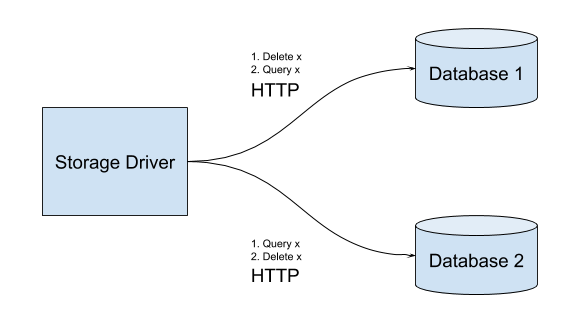
\includegraphics[width=0.75\textwidth]{simple_naive_polyglot.png}
\end{figure}

\subsection{Event Sourcing and OLEP}

The \textit{event sourcing} paradigm has been proposed as an approach to data modelling \ref{eventSourcing}, which is relevant to polyglot persistent. The idea behind it is to model the changes to the state as a log of events, instead of directly updating the database(s). Each event is then translated to one or more direct database operations. The event structure and the translation are defined by the developers and could be different in each case. The additional level of indirection results in a historical log of events that is much easier to interpret than just the final state. For example, a ``book-borrowed'' event in a library management system is much more descriptive to multiple out-of-context updates to some tables. Another advantage is that all or some of the updates could be ``replayed'' --- for example, if one is interested in a past state of the database, it could start from the beginning (or a known snapshot), and re-apply the events which happened in some period.

\textit{Online Event Processing (OLEP)}, as coined by Kleppmann et. al. \cite{OLEP}, is very similar. The difference between the two is mainly in the intent --- while the main focus of event sourcing is to make state changes easier to explain, audit and debug, OLEP uses the event log, and its properties, to keep the databases consistent. Online event processing also has similarities to the write-ahead log, used internally in many databases \ref{TODO} as means of ensuring durability.

A simplified diagram for the event-sourcing and OLEP-like architecture could be seen in figure \ref{figEventSourcingPolyglot}.

\begin{figure}[h]
    \caption{Simple event sourcing architecture combining two databases}
    \centering
    \label{figEventSourcingPolyglot}
    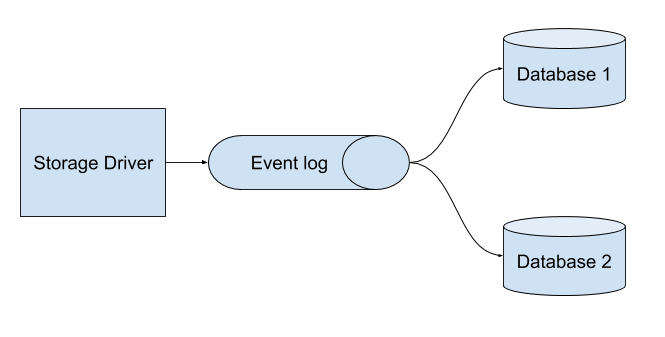
\includegraphics[width=0.75\textwidth]{simple_event_sourcing.png}
\end{figure}

Section \ref{prepOLEP} will explain the workings of event sourcing and OLEP, as well as their contribution to solving the consistency problems of polyglot systems.

\subsection{Read consistency in OLEP systems}

\section{Preparation}

\subsection{Consistency Guarantees and Transactions}
\label{trans}

All databases specify some guarantees that they give when users interact with them. Do writes take effect immediately? Can several operations run concurrently, and what can the outcomes be? The answers to those and many more questions are then used by developers to build quality applications that satisfy the requirements within the environment they operate in.

Transactions are the standard abstraction for consistency guarantees in many databases, most notably in relational ones \cite{wikiTrans}. Transactions encapsulate database operations in a consistent way, and provide the following properties:
\begin{itemize}
    \item Atomicity --- the operations in each transaction are either fully executed, or neither of them is. This means that if any one of them fails, the transaction won't change the visible database state at all.
    \item Consistency --- modifications by a transaction, performed on a database in a consistent state, will leave it in a consistent state.
    \item Isolation --- can concurrently running transactions cause inconsistency, and to what extent. Often there are multiple isolation levels.
    \item Durability --- once the effects of a transaction have been successfully saved in the database, they will persist even in the face of transient failures (e.g electricity outages).
\end{itemize}

The dissertation will specifically focus on the isolation property of a transaction. In practice, there are more than one isolation levels that storage systems offer. This is because often enforcing complete isolation comes at a performance cost which is too high. For the purpose of this work, the following isolation levels are of interest (from weak to strong) \cite{isolation}:
\begin{itemize}
    \item Read Uncommited
    \item Read Commited
    \item Snapshot Isolation
    \item Serializable
\end{itemize}

A transaction that spans several nodes (e.g servers) is a \textit{distributed transaction} \cite{wikiDistrTrans}. The performance cost of providing transactional semantics in a distributed environment is higher, because multiple nodes must be coordinated (and respectively more fault modes need to be covered).

\subsection{Existing Implementations of Polyglot Persistence}
\label{priorPoly}

As briefly mentioned in \ref{intro2pcsaga}, there are two main ways to implement polyglot persistence.

The first one is a synchronous extension of transactions in a monolithic storage system to a distributed architecture, using two-phase commit \cite{2pcWiki}. In this case, a global transaction manager sends a \textit{PREPARE} request containing the local transaction to each storage system, which on their turn reply with \textit{CAN COMMIT} or \textit{FAILURE}. If all storage systems reply with the former, that means that they will be able to commit even in the case of transient outages, once the manager asks them. In this case, the storage systems have also locked all fields that are read or updated, so that they remain unchanged by concurrent transactions. Then, the manager sends a \textit{DO COMMIT} message, which will make all storage systems persist the changes in the transaction. Otherwise, if any of the storage systems has replied with \textit{FAILURE}, the manager sends an \textit{ABORT} message, urging all to abort and roll-back the pending transaction.

The Saga pattern, on the other hand, is asynchronous in nature. The participating storage systems are updated sequentially, while the whole system continues to serve requests. If any of them fails, those that have previously reflected the changes need to roll back. This means that for every transaction that modifies the state, there must be a ``compensating transaction'' that undoes it for every storage system, in case any of the subsequent storage system fail while trying to apply the update.

\subsection{Online Event Processing --- OLEP}
\label{prepOLEP}

The Online Event Processing design was proposed by Kleppman, Beresford and Svingen in 2019 \cite{OLEP}. It describes a different architecture for handling polyglot persistence, that has its similarities with what's known as event sourcing \cite{fowEventSourcing} and CQRS (Command Query Responsibility Segregation) \cite{fowCQRS}.

At its core is the event log --- a durable, append-only data structure, which provides a holistic view of the data in our polyglot persistence system. Modifications to the single databases are only allowed through the log, in the form of ``events'' appended to it by producers. Databases then consume them, and reflect the changes locally. If any of them experiences a transient failure, it should continue from where it had stopped once it is back on. In this way, no reordering could occur across updates, as the event log provides a total order on them.

\subsection{Requirements Analysis}

The exact architecture will differ between applications, so all requirements are in the context of the demo chat application and its software infrastructure. The ideas described, however, must extend to general cases of polyglot persistence.

The polyglot persistence framework must be able to handle arbitrary number of databases. Because the architecture is dependent on the exact vendor and type of the database, I only consider databases from the following list:
\begin{itemize}
    \item PostgreSQL
    \item Lucene
\end{itemize}

They possible architectures must clearly define the isolation properties that they provide, together with a performance comparison between each other.

\subsection{Software Engineering Techniques}

\subsection{Starting Point}

\begin{thebibliography}{9}

\bibitem{netflixPolyglot}
\href{https://www.infoq.com/articles/polyglot-persistence-microservices/}{Polyglot persistence is used in Netflix's microservices architecture}

\bibitem{oneSize}
\href{http://cs.brown.edu/research/db/publications/fits_all.pdf}{M. Stonebraker and U. Çetintemel: ``One Size Fits All'': An Idea Whose Time Has Come and Gone }

\bibitem{polyglotWiki}
\href{https://en.wikipedia.org/wiki/Polyglot_persistence}{Wikipedia: Polyglot persistence}

\bibitem{polyglotMartin}
\href{https://martinfowler.com/books/nosql.html}{Pramod J. Sadalage and Martin Fowler: NoSQL Distilled --- Chapter 13. Polyglot Persistence}

\bibitem{neo4jTransactions}
\href{https://neo4j.com/docs/java-reference/current/transaction-management/introduction/}{Neo4J documentation: Introcution to Transaction management}

\bibitem{flexcoin}
\href{http://hackingdistributed.com/2014/04/06/another-one-bites-the-dust-flexcoin/}{NoSQL Meets Bitcoin and Brings Down Two Exchanges: The Story of Flexcoin and Poloniex}

\bibitem{2pcsaga}
\href{https://developers.redhat.com/blog/2018/10/01/patterns-for-distributed-transactions-within-a-microservices-architecture/}{Patterns for distributed transactions within a microservices architecture: RedHat Developer Blog}

\bibitem{OLEP}
\href{https://queue.acm.org/detail.cfm?id=3321612}{Martin Kleppmann, Alastair R. Beresford, and Boerge Svingen: Online Event Processing}

\bibitem{wikiTrans}
\href{https://en.wikipedia.org/wiki/Database_transaction}{Wikipedia: Database transaction}

\bibitem{wikiDistrTrans}
\href{https://en.wikipedia.org/wiki/Distributed_transaction}{Wikipedia: Distributed transaction}

\bibitem{isolation}
\href{https://www.microsoft.com/en-us/research/wp-content/uploads/2016/02/tr-95-51.pdf}{A Critique of ANSI SQL Isolation Levels}

\bibitem{2pcWiki}
\href{https://en.wikipedia.org/wiki/Two-phase_commit_protocol}{Wikipedia: Two-phase commit protocol}

\bibitem{fowEventSourcing}
\href{https://martinfowler.com/eaaDev/EventSourcing.html}{Event Sourcing by Martin Fowler}

\bibitem{fowCQRS}
\href{https://martinfowler.com/bliki/CQRS.html}{Command Query Responsibility Segregation (CQRS) by Martin Fowler}

\end{thebibliography}

\end{document}